% first pages of the pdf of the thesis that will submitted

\newcommand{\thesistitle}{Scientific machine learning in physics: symmetries, PINNs and applications in nanophotonics}
\pagestyle{empty}

%-----------------------------------------------
% Page 1: Cover page
%-----------------------------------------------

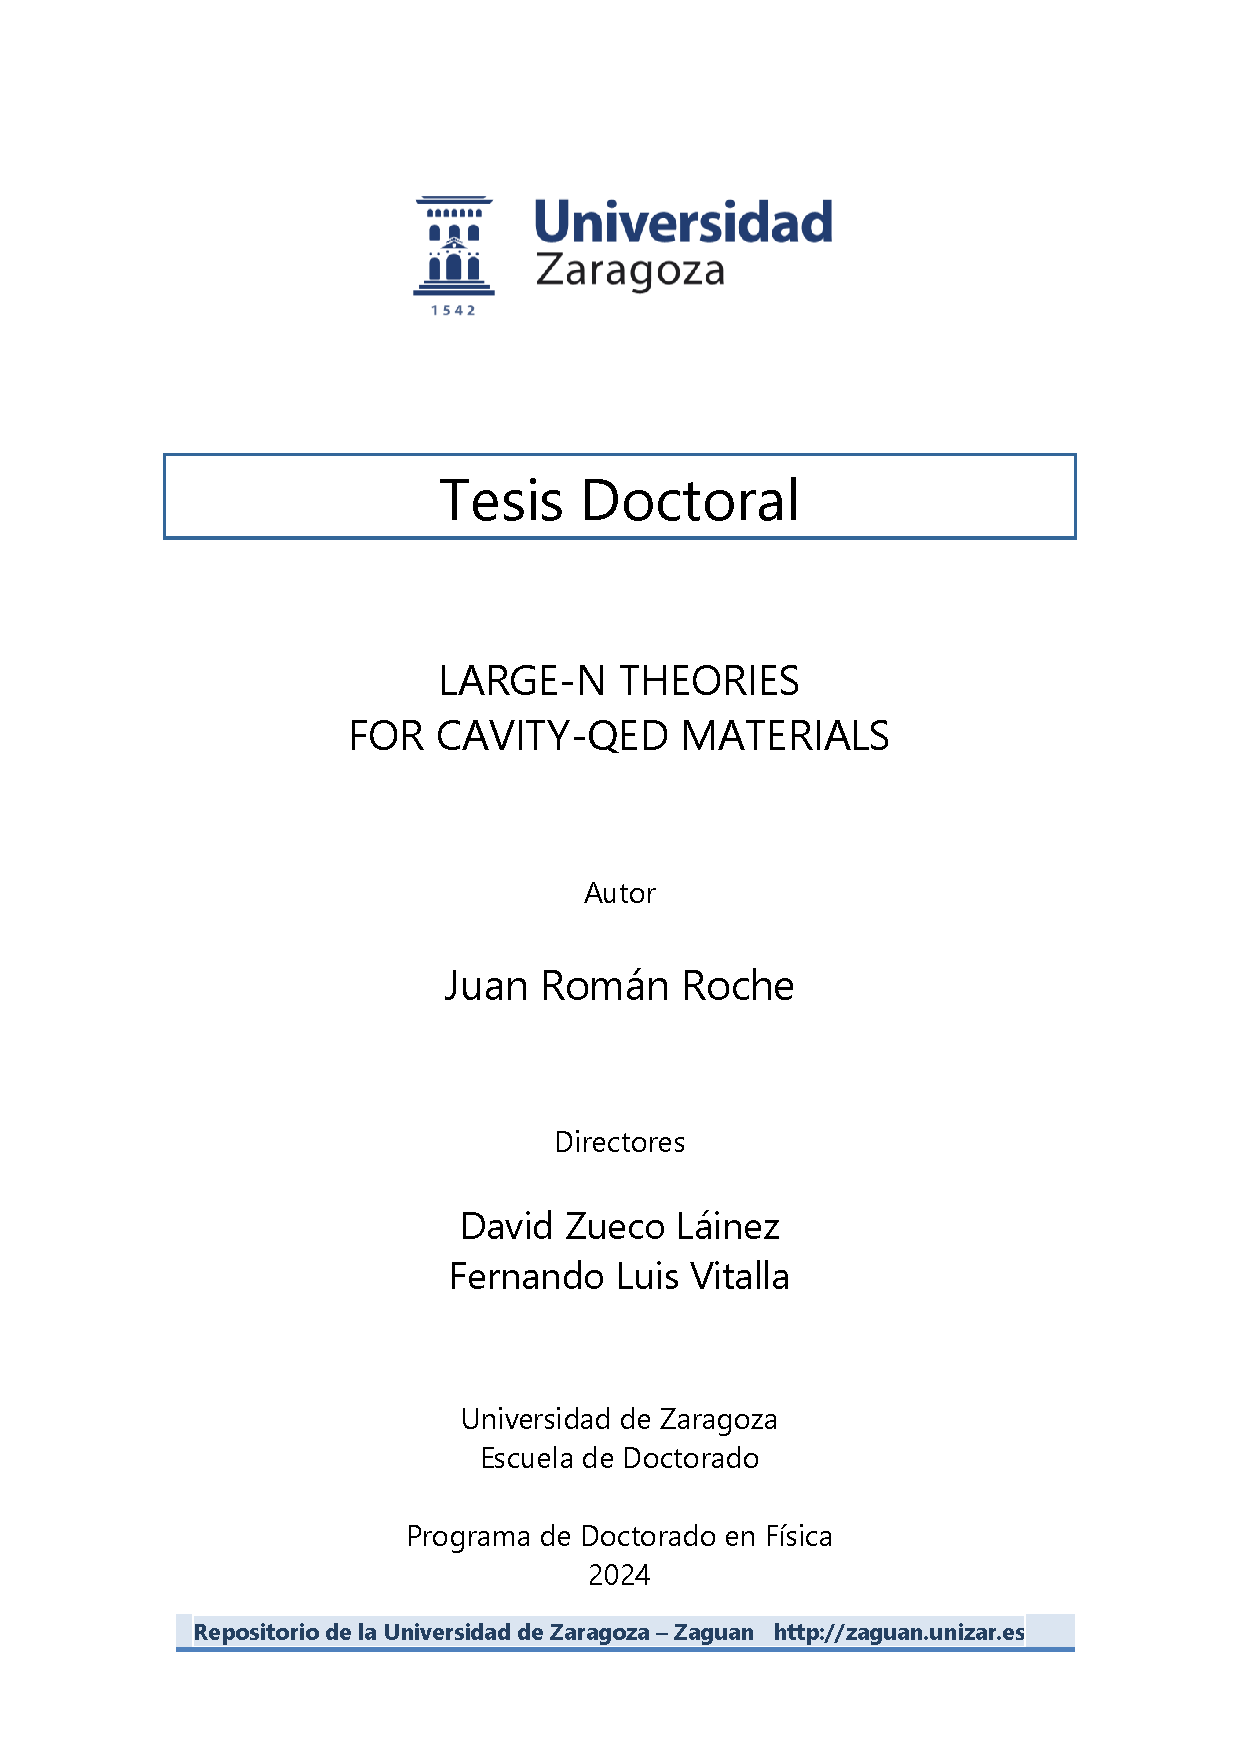
\includepdf{frontbackmatter/portada_normalizada.pdf}

%-----------------------------------------------
% Page 2: Blank
%-----------------------------------------------

\
\newpage

% %-----------------------------------------------
% % Page 3: Quote or dedication
% % It is adviced to include something here, otherwise this page is completely removed (not even left blank) and the table of contents start right after the credits and copyright which looks weird.
% %-----------------------------------------------

% \vspace*{15mm}
% \begin{quotation}
% \begin{flushright}
% {\bf \em Dedicatoria ...}
% \end{flushright}
% \end{quotation}

% \newpage

% %-----------------------------------------------
% % Page 4: Blank
% % Only present if Page 3 is included
% %-----------------------------------------------
% \
% \newpage


%-----------------------------------------------
% Table of contents
%-----------------------------------------------

\pagestyle{toc}
\hypertarget{toc}{} % so that we can link back to toc from pages
\tableofcontents 
\newpage
\pagestyle{regular}
